\chapter{系統架構與實作}

    本研究所設計之系統,利用超聲波對麥克風造成的非線性響應輸出,與主動式噪音控制消除高關聯度噪音等特性。
嘗試解決在部署麥克風干擾器的場域裡,無法取得有效聲學紀錄的問題。
同時借鏡密碼系統的機密性與不可否認性,發展一套於會談結束後,以其為基礎的會談錄音存取控制機制。
透過上述機制的結合,能夠使在部署超音波麥克風干擾器的會談情境中,於會談結束後,允許特定參與者得以取得有效之聲音記錄。

\section{系統架構}

\begin{figure}[H]
    \centering
    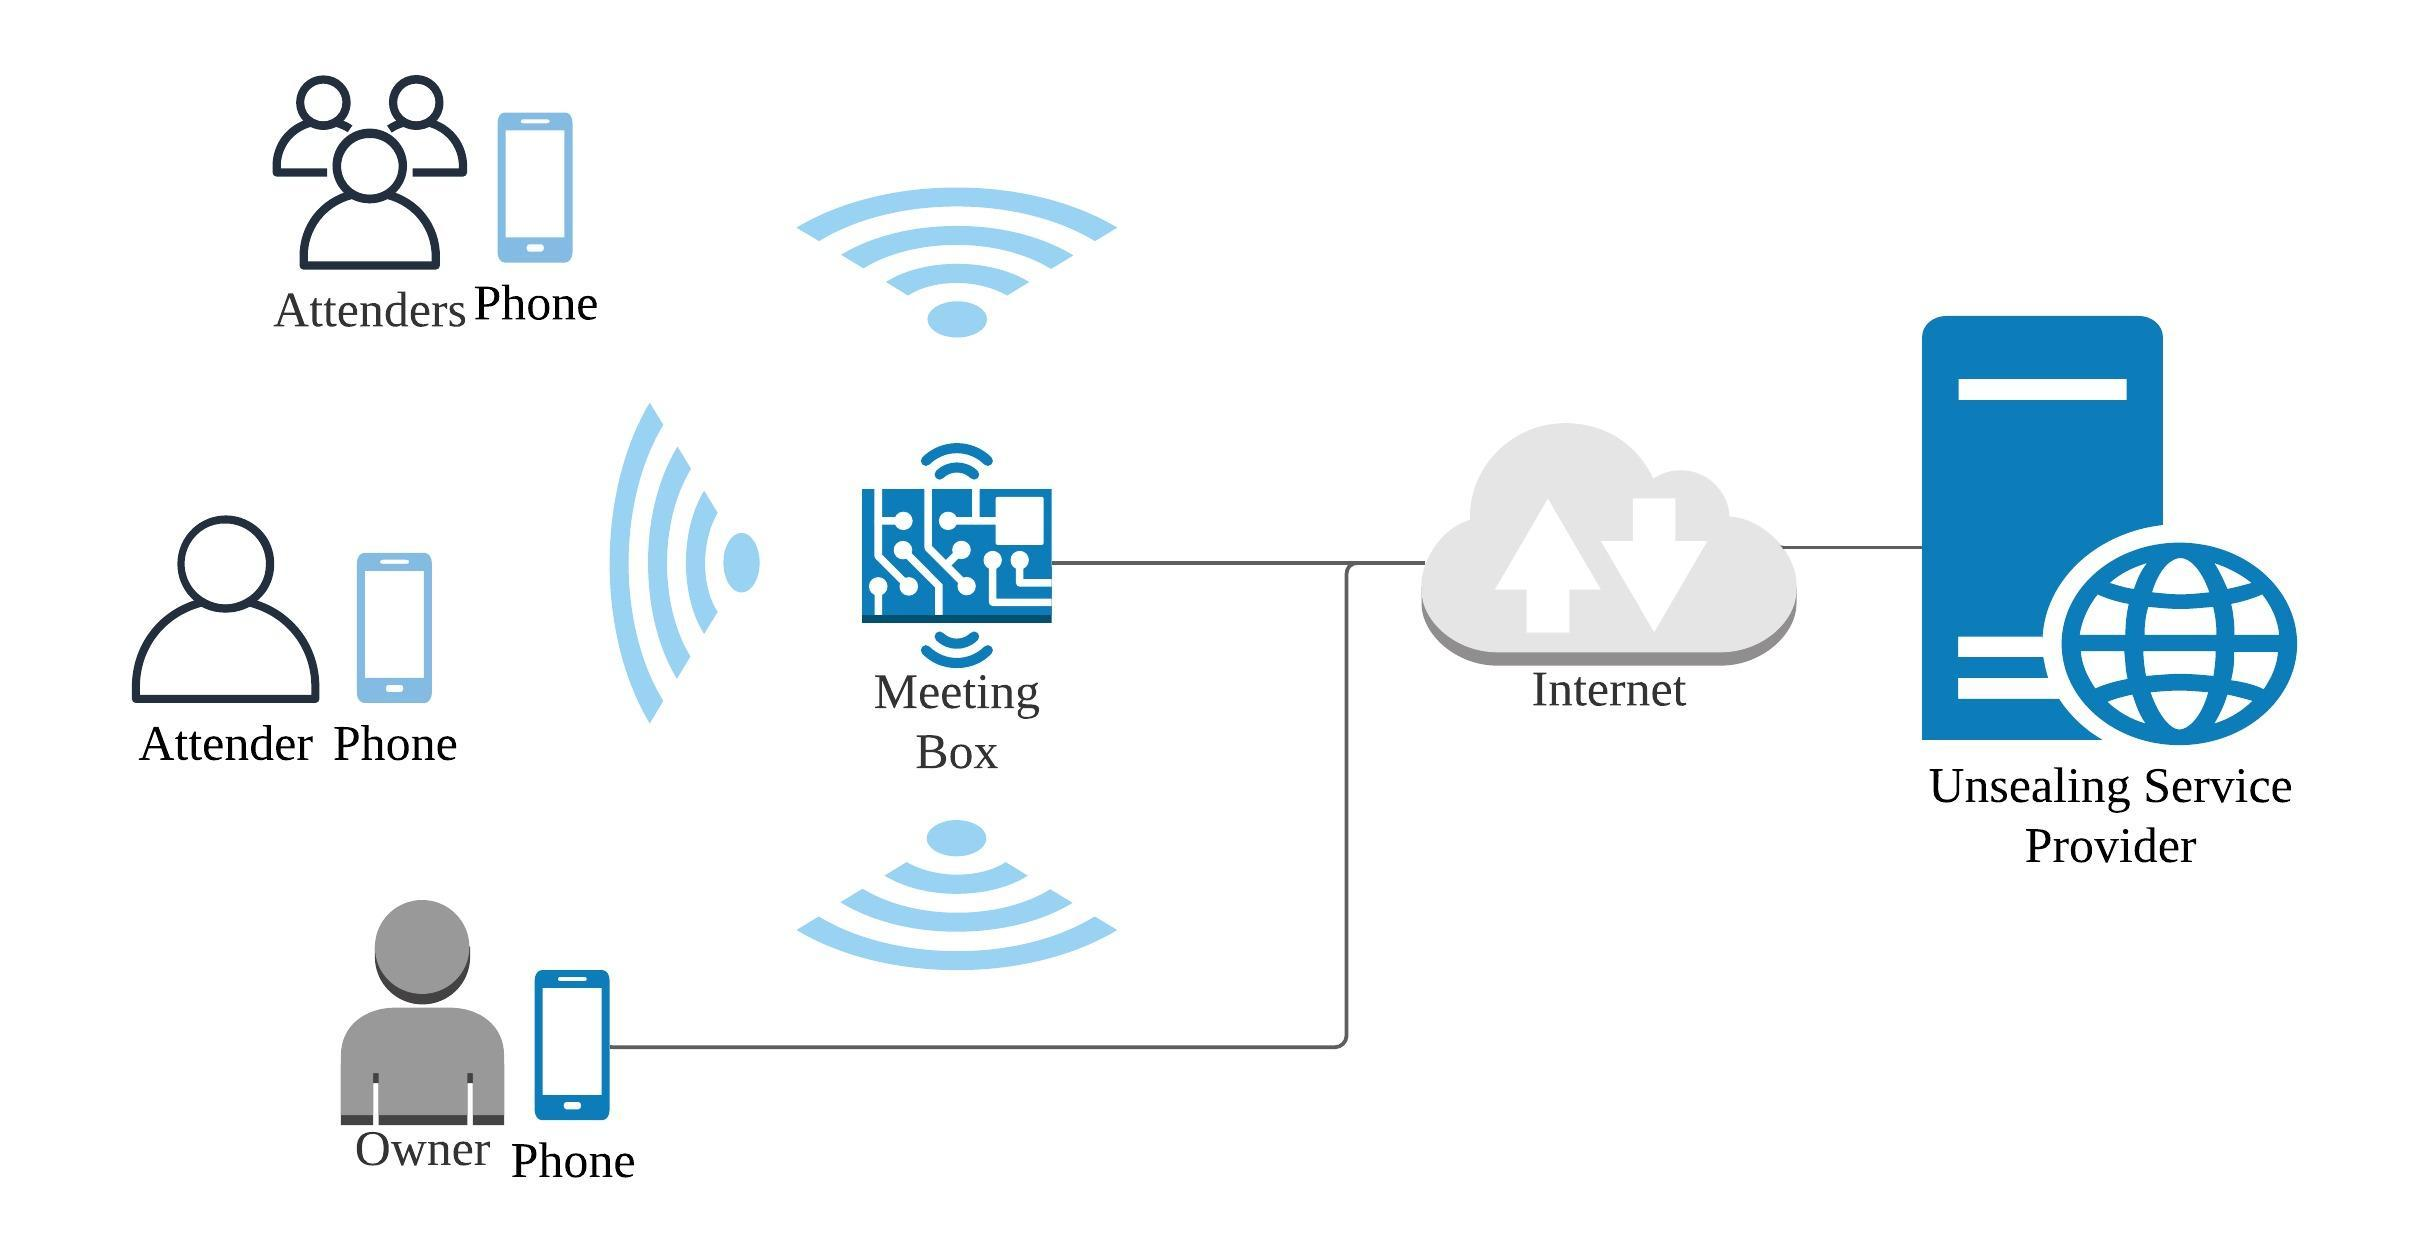
\includegraphics[width=0.8\textwidth]{single-owner-architecture}
    \caption{單一 Owner 系統架構圖}
    \label{fig.s-o-arch}
\end{figure}

    本系統由 $MeetingBox$、$Server$ 以及會談參與者 ($Owner$、$Attender$) 所組成。
各會談的會談參與者 ($Owner$、$Attender$) 僅定義於當次會談,每次會談的會談參與者角色 ($Owner$、$Attender$) 可為不同群體。
會談參與者 ($Owner$、$Attender$) 於 $MeetingBox$ 的周圍進行會談,並可以與其操作互動來控制會議的開始與終止。
$MeetingBox$ 在會談進行中開啟超聲波麥克風干擾器,因此鄰近的麥克風或周邊的聲音記錄裝置,都將因受到干擾而失效,無法有效記錄會談內容。

    $MeetingBox$ 於會談進行中持續紀錄聲音,內容為受到超聲波麥克風干擾器干擾的會談錄音 ($REC_{J}$)。
於會談結束後,受超聲波麥克風干擾器干擾的會談聲音記錄 ($REC_{J}$) 將透過本研究所設計的「解封」 (Unseal) 機制,
使會談參與者 ($Owner$、$Attender$) 中的會談擁有者 ($Owner$),得以取得已解封 (Unsealed) 的有效聲音記錄 ($REC_{rev}$)。

\subsection{$Owner$}

    會談參與者 ($Owner$、$Attender$) 中,$Owner$ 屬於 $Attender$,為 $Attender$ 的子集合,
$Owner$ 定義為 $Attender$ 中的特權角色。
$Owner$ 於會談結束後,有能力決定是否解封(Unseal)會談聲音記錄,並獲取已解封 (Unsealed) 的有效聲音記錄 ($REC_{rev}$)。
$Owner$ 可以是一或多人。當會談中只有一個 $Owner$ 時,系統架構如圖 \ref{fig.s-o-arch} 所示。
當會談中有多個 $Owner$ 時,系統架構如圖 \ref{fig.m-o-arch} 所示。

    $Owner$ 持有智慧型手機,用來與$MeetingBox$ 互動,獲取 $MeetingBox$ 上的資訊,並有能力於會談進行中、會談結束後,
與 $Server$ 通訊,執行本研究所設計的系統機制「註冊會議擁有者」 (Register Owner) 與「解封」 (Unseal)。
上述 $Owner$ 獲取 $MeetingBox$ 資訊的方法,本研究以掃描 QR Code 為例。

\begin{figure}[H]
    \centering
    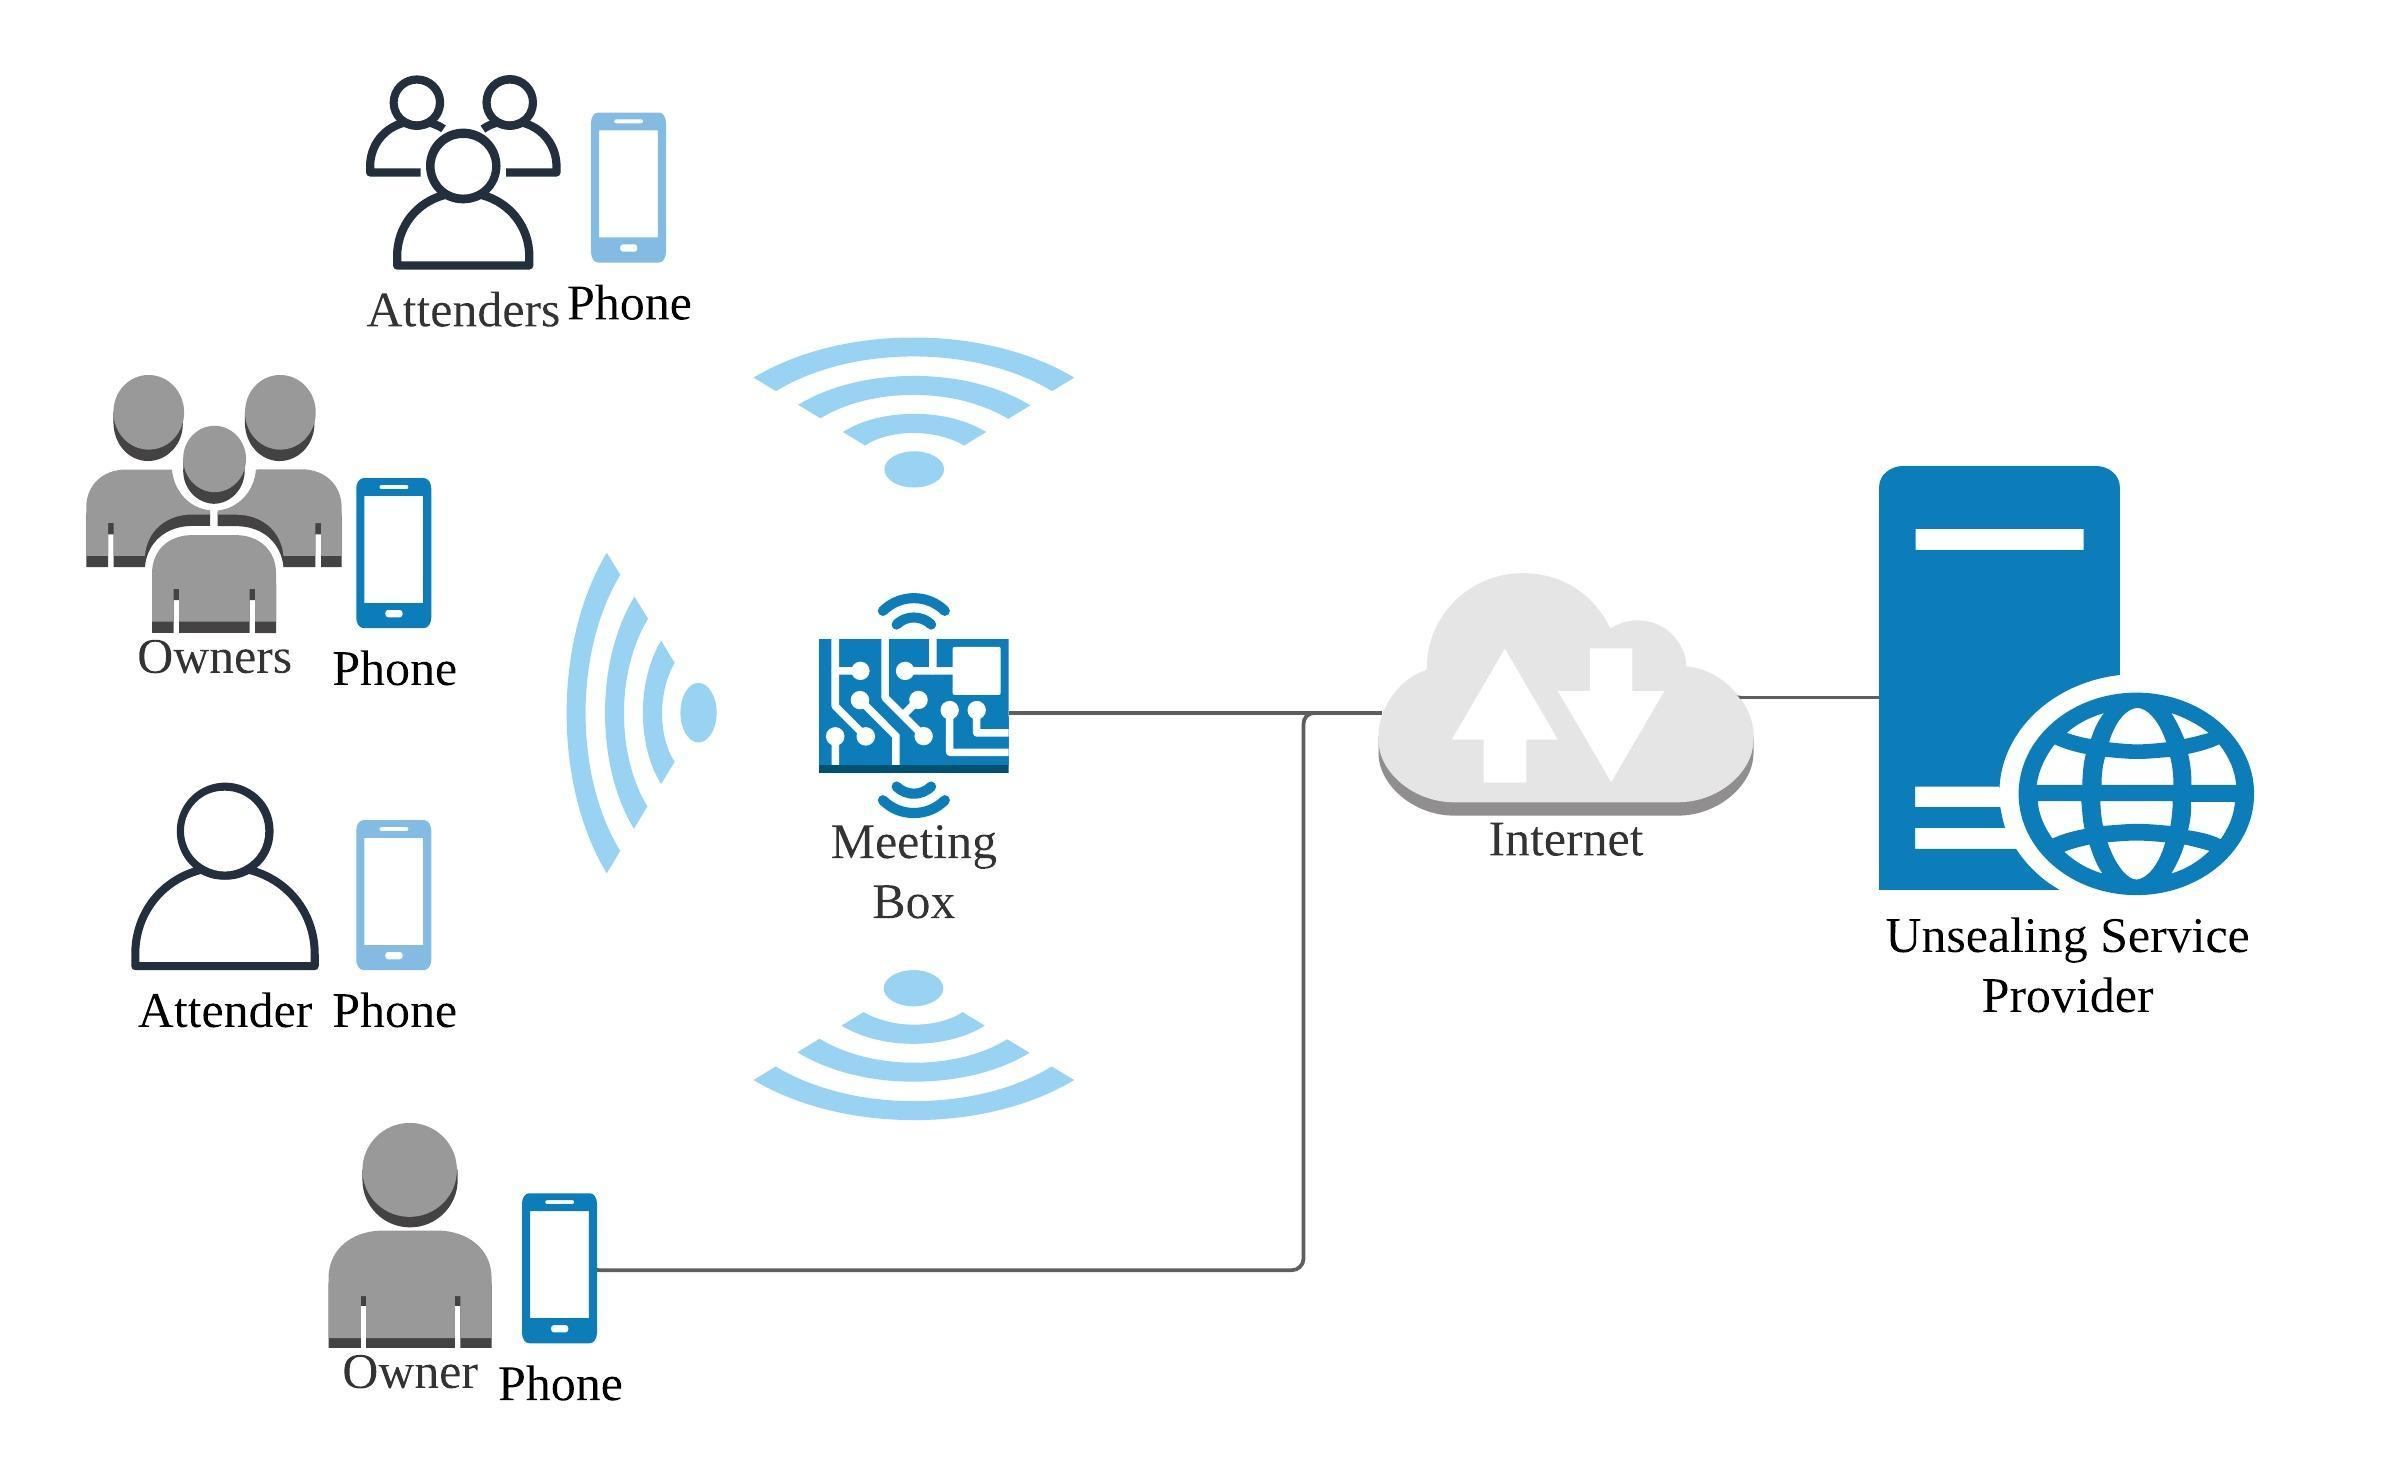
\includegraphics[width=0.8\textwidth]{multi-owner-architecture}
    \caption{多 Owner 系統架構圖}
    \label{fig.m-o-arch}
\end{figure}


\subsection{$Attender$}
\subsection{$MeetingBox$}

    {$MeetingBox$} 裝置包含下列組件:
    \begin{enumerate}
        \item 超音波麥克風干擾器。
        \item 具有 QR Code 顯示功能的螢幕。
        \item 實體按鈕,供會談參與者操作與互動。
    \end{enumerate}

\subsection{$Server$}


\section{符號定義}

    本研究設計之系統所使用符號與其意義如表 \ref{table:tab.symbol} 所示。

\begin{table}[H]
    \centering
    \caption{符號定義表}
    \label{table:tab.symbol}
    \begin{tabular}{ c c }
        \hline
        \bf{符號} & \bf{釋義} \\
        \hline
        $REC_{J}$ & 已被超聲波麥克風干擾器干擾的會談之聲音記錄 \\
        $REC_{N}$ & 超聲波麥克風干擾器於麥克風的響應輸出之聲音記錄 \\
        $REC_{rev}$ & 解封後(Unsealed)的會談聲音記錄 \\
        $time_{Max}$ & 會談進行時間長度的最大值、$REC_{N}$ 的時間長度 \\
    \end{tabular}
\end{table}

\section{系統流程}

\section{系統機制}

\subsection{錄音存取控制與解密}

\subsection{主動式噪音控制}

\subsection{樣本對齊}

\section{系統實作}